\section{Durchführung}

    Zur Messung der Wellenlänge und des Brechungsindexunterschiedes wird der folgende Versuchsaufbau verwendet.

    \begin{figure}
        \centering
        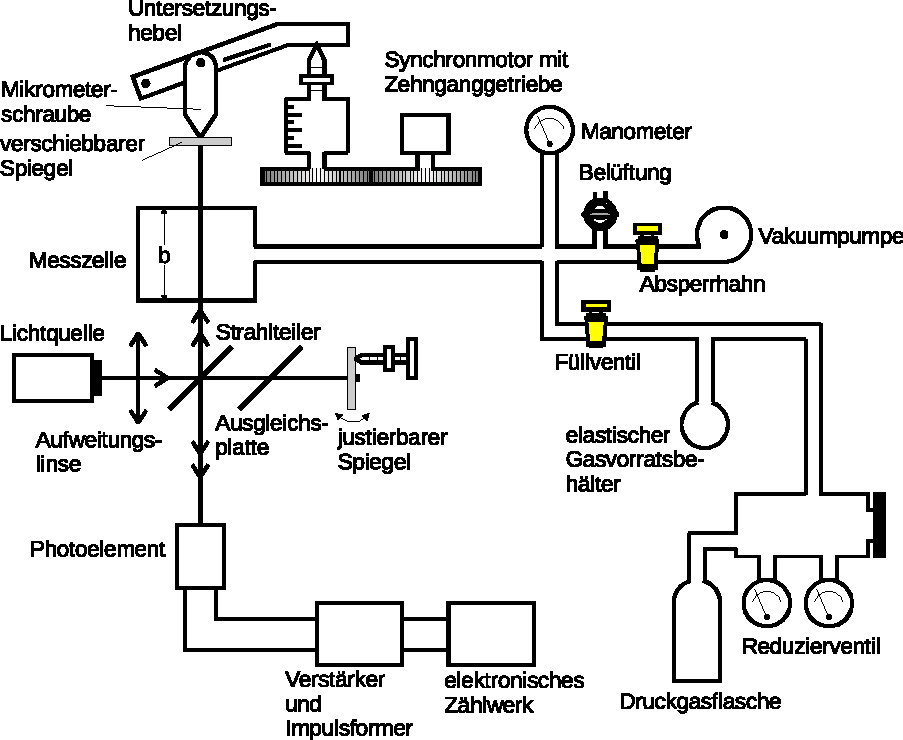
\includegraphics[width=\textwidth]{content/img/Abb_7_edit.pdf}
        \caption{Der Versuchsaufbau des Interferometers zur Messung von Wellenlänge und Brechungsindexunterschied.}
    \end{figure}

    In diesem Experiment dient ein Laser mit der Wellenlänge $\lambda = \SI{635}{\nano\meter}$ als Lichtquelle.
    Eine Linse hinter dem Laser weitet den Stahl auf.\\
    Zu Beginn der Messung muss der Strahlengang des Lichts ausgerichtet werden.
    Dazu werden mithilfe des justierbaren Spiegels die beiden hellsten Lichtpunkte,
    welche am Detektor auf einem Stück Papier sichtbar gemacht werden,
    zur Deckung gebracht.
    Eine Zerstreuungslinse auf der Strecke zwischen der semipermeablen Platte P (hier Strahlteiler genannt) und dem Photoelement vergrößert das Bild.
    Das Interferenzbild muss abschließend noch so ausgerichtet werden,
    dass das Zentrum auf den Eintrittsspalt der Photozelle trifft.
    Das Photoelement misst elektrische Impulse,
    die von den Intensitätsmaxima erzeugt werden und zeigt sie mithilfe eines Selektivverstärkers der Übersetzung 1:5,017 
    und eines Impulsformers auf einem elektrischen Zählwerk an.\\
    \\
    Zur Messung der Wellenlänge wird nun ein Motor angeschaltet,
    welcher dazu dient,
    mit der Mikrometerschraube den verschiebbaren Spiegel gleichmäßig zu verschieben.
    Es wird eine Verschiebung von $\symup{\Delta}d = \SI{5}{\milli\meter}$ gemessen,
    wobei mindestens 3000 elektrische Impulse regristriert werden sollten.
    Die Messung wird zehnmal wiederholt,
    wobei der Spiegel zwischen den Intervallen von $\SI{5}{\milli\meter}$ noch einen halben Millimeter in die jeweilige Richtung verschoben werden sollte, 
    damit die $\SI{5}{\milli\meter}$ bei einer begrenzt langen Mikrometerschraube bei jeder Messung sicher erreicht werden.
    Es wird die Zahl $z$ der gezählten Intensitätsmaxima (also die elektrischen Impulse) auf dem Zählwerk notiert.
    Die Wellenlänge kann mithilfe der Gleichung \eqref{eqn:Wellenlänge} berechnet werden.\\
    \\
    Um den Brechungsindexunterschied zu bestimmen,
    wird der verschiebbare Spiegel zunächst in die Ausgangsposition zurückbewegt.
    Dann wird mithilfe einer handbetriebenen Vakuumpumpe ein Druck $p'$ in der Messzelle erzeugt.
    Dabei muss darauf geachtet werden,
    dass sich der Druck nicht zu schnell verändert,
    da sonst nicht alle Intensitätsmaxima vom Photoelement wahrgenommen werden können auf dem Zählwerk angezeigt werden.
    Nachdem $p'$ in der Messzelle erreicht ist,
    wird $p'$ und die Zahl $z$ der elektrischen Impulse notiert.
    Dann wird der Druck wieder auf den ursprünglichen Druck $p$ reguliert,
    wobei auch hier darauf geachtet werden muss,
    dass sich der Druck nicht zu schnell verändert und alle Intensitätsmaxima gezählt werden können.
    Wenn $p$ erreicht ist,
    werden $p$ und $z$ notiert.\\
    Die Messung wird fünfmal wiederholt und der Brechungsindexunterschied kann mithilfe der Gleichung \eqref{eqn:Brechungsindex} berechnet werden.
